\chapter{6. Conclusion}

\section{Future Work}

This is the 



\subsection{safer route navigation}
Utilizing the data collected by the users, we can make a routing system based on safeness within the roads.

Modern map services enables custom path finding, where applications can set different weights for each road segment. Improving the overall bike experience will introduce people to ride their bikes more frequently, causing less cars.
The ring bell Geo location data having weights good and bad, the paths can alter to take a safer route. This will incentives the users for using the app.
In addition, the reported data can be sourced to car navigation systems to let car drivers notice places that are bike heavy.



\subsection{VR for non bikers}

\begin{marginfigure}[{2cm}]
 	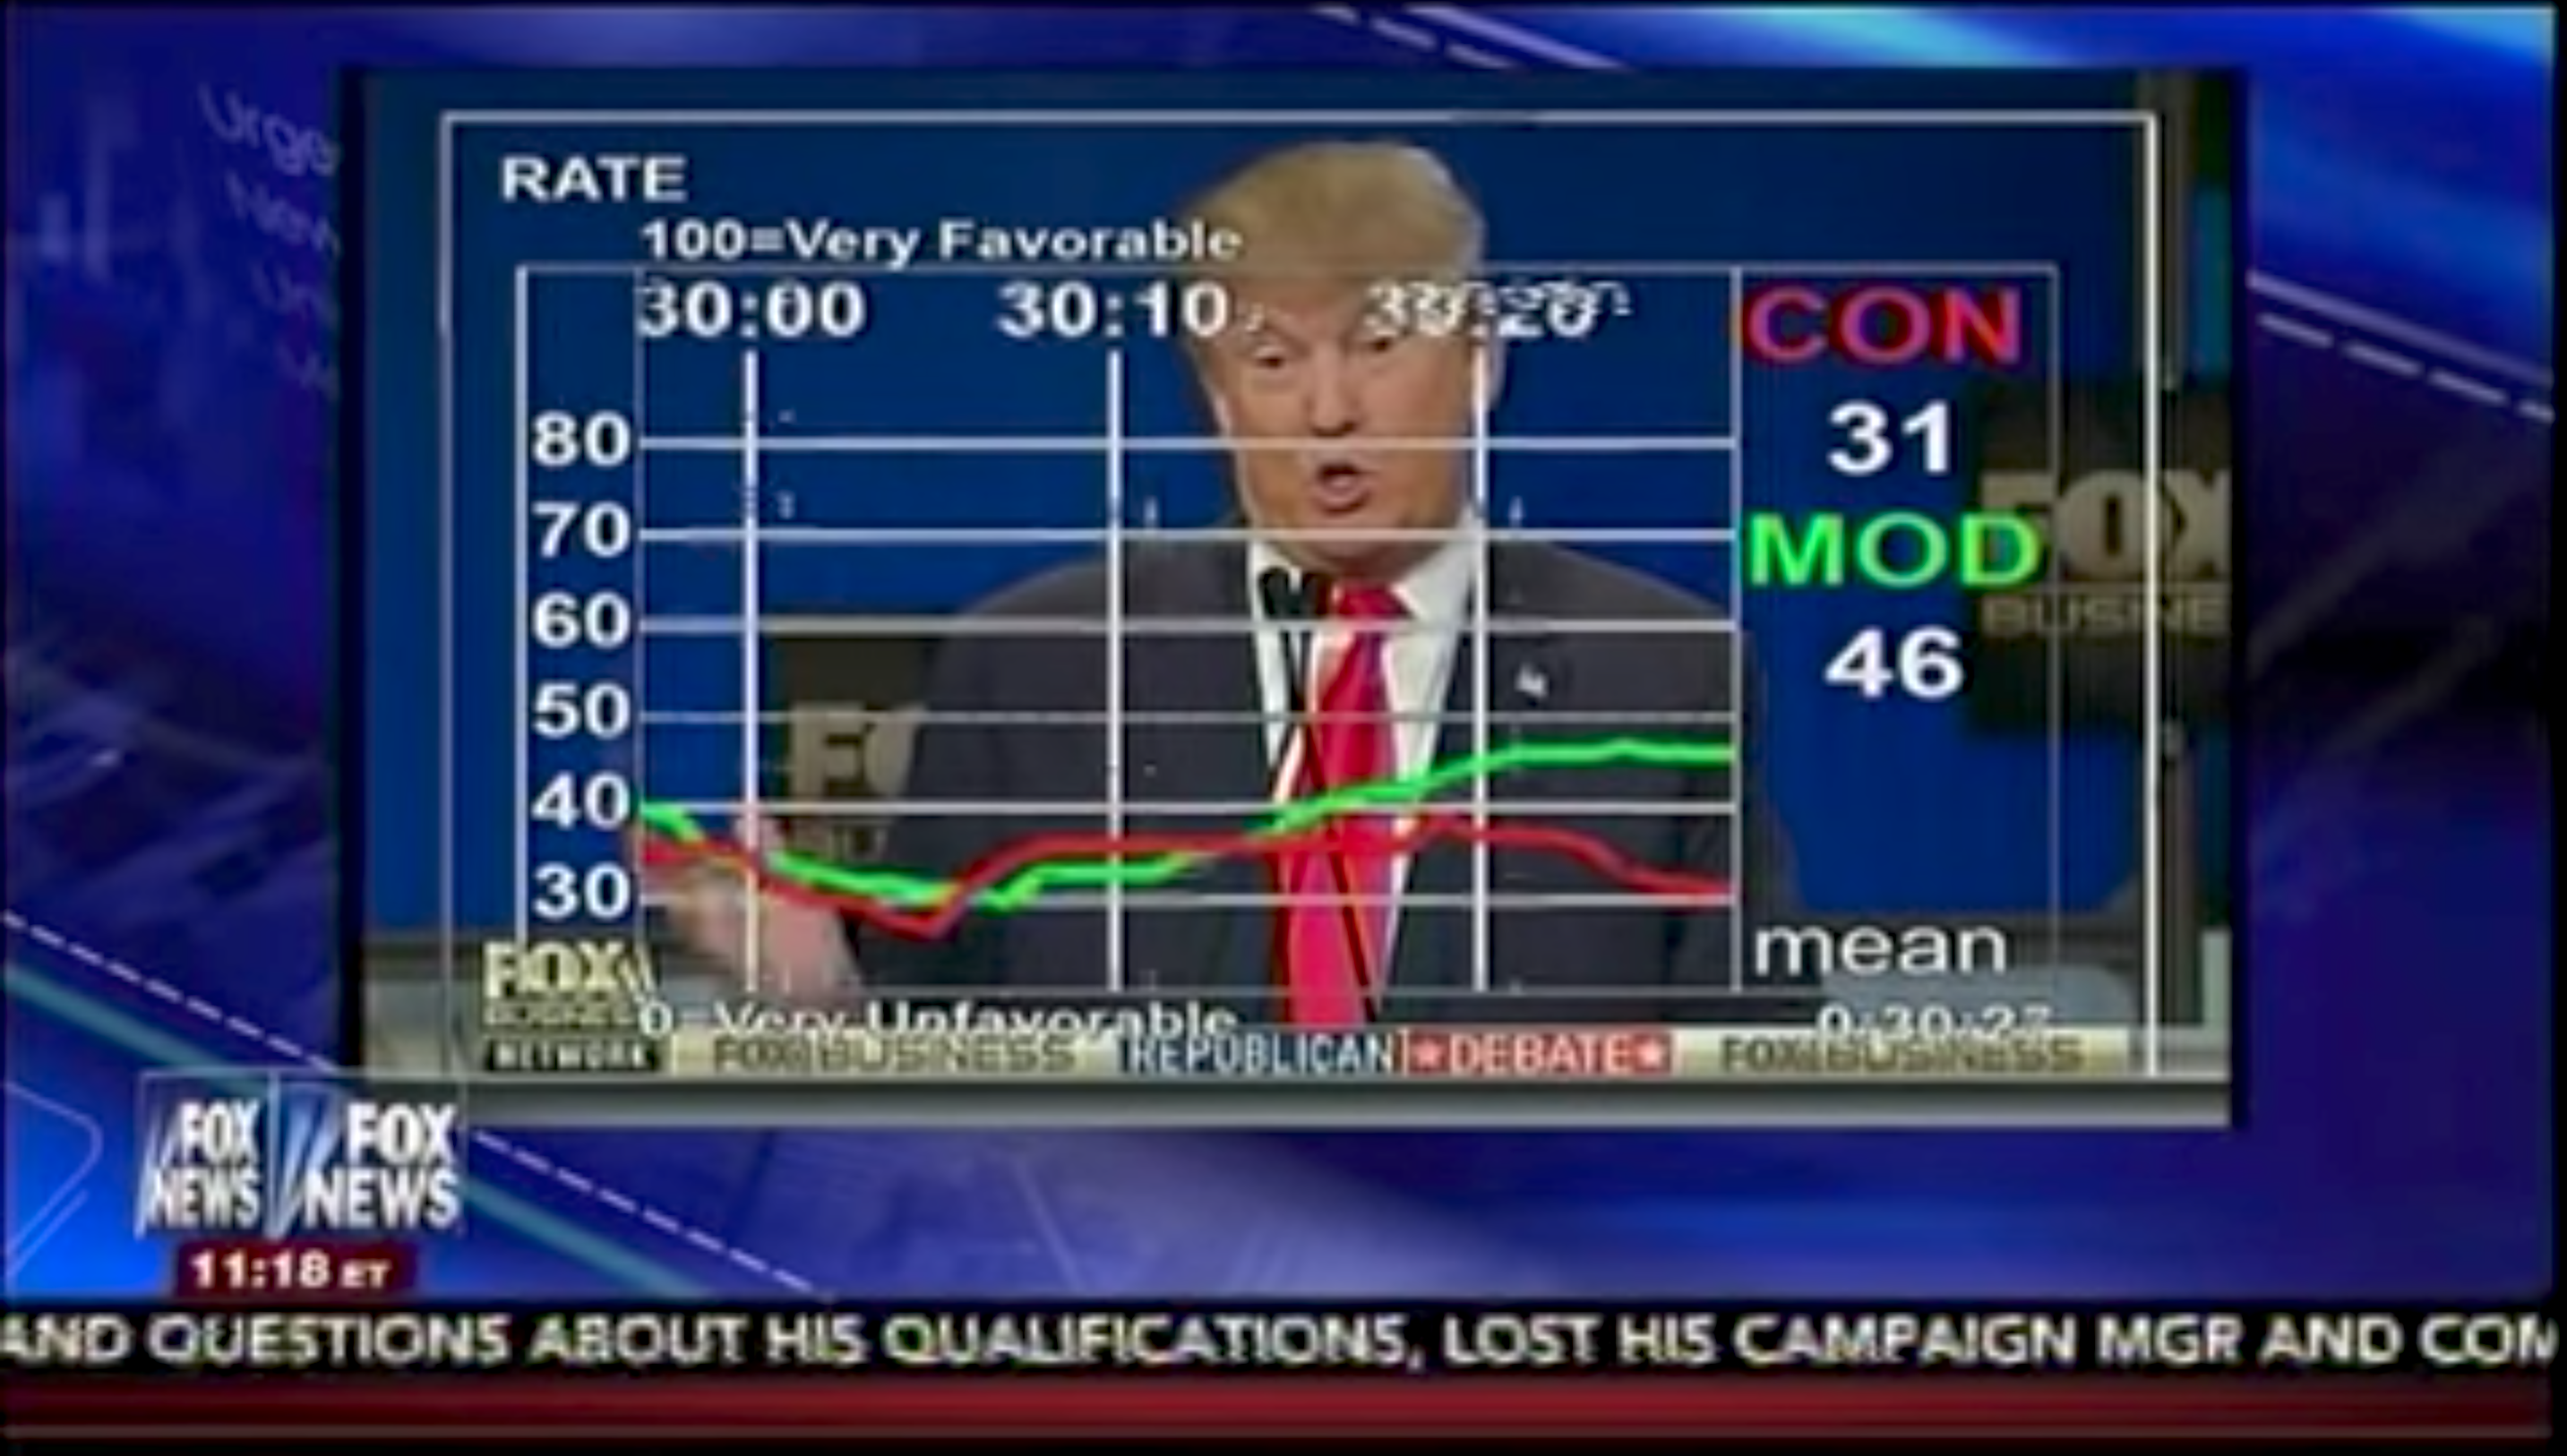
\includegraphics[width=\textwidth]{chapters/6/fig/pollester.png}               
 	 \caption{method for continuous input}
  	\label{fig:poll}
\end{marginfigure}
This app had focused on bikers, and did not take into account people who use other modes of transportation, such as pedestrians or car drivers. It is important to incorporate input from diverse people, and this both applies to the analytical and synthetic phase. It is easy to imagine to discuss the prioritization side, but the data on on-bike reports be should capture in a simulated environment.
Using a VR headset can simulate the bike ride and solicit data from people using a virtual environment projecting recorded material of one commute.

\subsection{Incentivasation}
Shirkey has mentioned the internet have lowern There are two kinds of value mechanisms in a collective action. \cite{shirky2010cognitive}
distributed donation matching system \\
method for periodic participation - donation matching system \\
% combining for post / pre natural / artificial disasters
\subsection {update infrastructure for autonomous vehicles}
use this renovation opportunity for making cities compatible with autonomous vehicles (PEV)
\subsection{Headphones w/ noise cancellation for collecting sound from both
sides}
% TODO: incomplete
\subsection{Holacracy and liquid democracy}
% TODO: incomplete

\section{Concluding Remarks}
\cite{rudofsky1964architecture}


 